
\section{IoT \& Big Data Platform}

Challenges of WAZIUP will be tackled using an open IoT-big data platform with affordable sensors connected through an IoT-Cloud open platform.
This platform will also make use of mobile phones and real-time processing to empower users and deliver the needed services.
The project will not develop any new IoT/Big Data software platform, but, rather exploit the existing solutions and adapt them for the purpose. Hereafter a compact list of core technical functionalities encompassed by the platform:

\begin{itemize}
   \item \emph{Cloud-based real-time data collection combined with analytics and automation software:} thus, the platform will offer cost-effective solutions for aggregating different machines and sensor types to engender efficiency, smart automation and optimization in the rural context.
   \item \emph{Intelligent analytics of sensor and device data:} studied in order to optimize for performance of the rural workplace, detect potential outages, and finally reduce overall maintenance costs.
   \item \emph{Integration to 3rd parties' platform:} enables customers' benefit of scaling fast and easy.
   \item \emph{PaaS (Platform-as-a-Service) provider:} WAZIUP will provide to business clientele with independently maintained platform upon which their web application, services and mobile applications can be built.
\end{itemize}

\subsection{Platform overview}


\begin{figure}[h!]
\centering
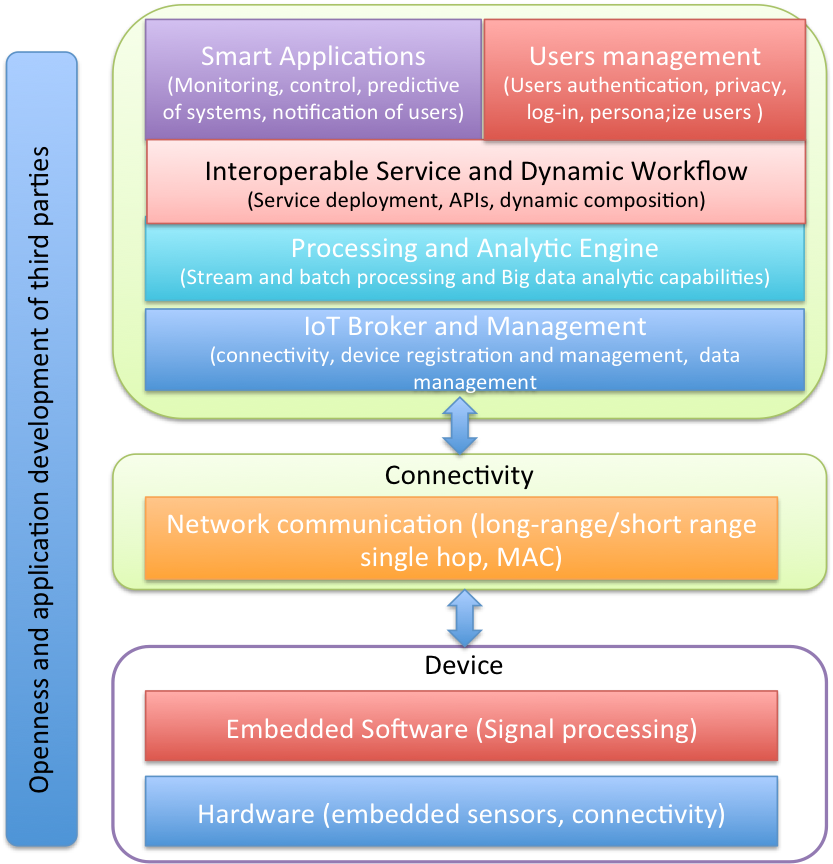
\includegraphics[width=0.7\textwidth]{figs/functional.png}
\caption{Functional overview of WAZIUP}
\label{fig:func}
\end{figure}

The Figure~\ref{fig:func} displays the functional overview of WAZIUP.
The topmost block represents the Cloud platform, the middle one is the network connectivity while the bottom one is the local deployment, including gateway and sensors.

\subsection{IoT platform}

\subsubsection{IoT architecture overview}


\begin{figure}[h]
\centering
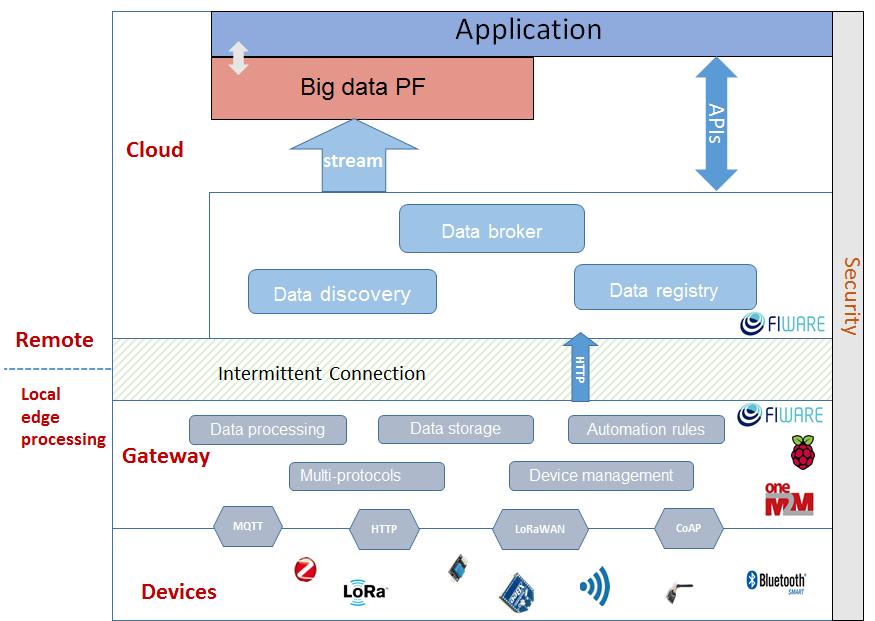
\includegraphics[width=\textwidth]{figs/iotarchi.png}
\caption{IoT platform architecture}
\label{fig:iotarchi}
\end{figure}

Our iot platform architecture is presented in Figure~\ref{fig:iotarchi}.
It has three main layers: device layer, gateway layer and the cloud layer.

\begin{itemize}
  \item \emph{The device layer}
    It includes IoT sensors and actuator that are able to communicate each on its protocol (MQTT, CoAP, HTTP, LoRAWAN) with the gateway. It a constraint and autonomous device. Considering the project circumstances it has to be low cost and doesn’t consume much power.
  \item \emph{The gateway layer}
  The gateway is a key component in our architecture since it ensure a secure bidirectional communication between the Iot devices and the cloud services. It interfere with various kind of devices: getting the data from sensors and sending commands to actuators.
  It has to be multi-protocol in order to be able to support diverse devices and it need to have device management capabilities.
Since the connection is intermittent in our project, it is mandatory that the gateway is able to manage local rules (for example some event processing), to store data locally and to have low speed internet connectivity (2G: GPRS, EDGE).
  \item \emph{The cloud layer}
  Our cloud main component are: the Data broker, the data registry and the data discovery.
  \item \emph{Data broker:}
    it is the key component of the IoT cloud services, it is based on publish/ subscribe mechanism to ensure data transfer from different producers to their respected consumers.
  \item \emph{Data registry:}
    it contains the virtual representation of devices (the data and the meta-data)
  \item \emph{Data discovery:} 
    it is responsible on querying the data.
\end{itemize}

\subsubsection{IoT components}

\todo{Explain the functional role of the different IoT components (IoT broker, IoT bridge..)}


\subsubsection{Technology and tools}

In this section we will present our main tools and technology that we will be using to reach our project objectives.
First, To fulfill our architecture requirements on the gateway and cloud level, FIWARE project is a good candidate.
It is open source and it has multiple components that can be used in our project.
In the cloud level the Orion context broker is the all-in-one solution containing the data broker, data registry and discovery components.
It is based on the Next Generic Service Interfaces (NGSI) 9/10.
NGSI specification defines a data model and interfaces to manage the whole cycle of the virtual entities.  

In the gateway level:
\begin{itemize}
  \item Cepheus enabler can be an option for the “local rules” component since it has a complex event processing engine. 
  \item IoT agent: can be an option to ensure the multiprotocol characteristic. Each IoT agent can be responsible on the data transfer to and from the devices using the device specific protocol. 
\end{itemize}

Second, to fulfill our requirement on the devices and networking level, LoRa technology captured our attention.
It specifies LoRaWAN for Low Power Wide Area Network (LPWAN), the kind of technology needed in our project context (rural environment).
Using LoRaWAN we can reach above 20 km in Line-Of-Sight (LOS) condition between the  device and the gateway. 


\subsubsection{Deployment}

\todo{Present the local, remote cloud.? resin}


\subsection{Big Data Platform}

\todo{Charlotte}

\subsubsection{Big Data Platform overview}


\subsubsection{Review of Big Data tools}


\cdu{to be moved to related works?}
Far from an exhaustive list, this paragraph describes the most used Open Source Big Data tools and compares them in order to give a better understanding of the Big Data ecosystem. Moreover, this review gives an indication on the best tools fitted for WAZIUP platform. 


\paragraph{Databases and data warehouses}

HDFS, developed by Apache, is a distributed, scalable and portable file-system written in Java for the Hadoop Framework.
It has been designed for large dataset analysis and by its structure has high fault tolerance. It is the basis upon which everything works in the Hadoop Ecosystem.
Build on top of HDFS, Apache HBase is a distributed, non-relational column oriented datastore.
HBase is designed to efficiently address random access and fast record lookup.
It has the capability to handle extremely large tables of data with low latency.
Though, this data storage tool should be used when random and real-time read/write access to data is needed and when many thousands of operation per seconds need to be performed on large datasets (up to petabytes).
Apache Hive is a data warehouse infrastructure that can manage and query unstructured data as if it were structured.
As a full component of Hadoop Ecosystem, it uses MapReduce for execution and HDFS for storage.
It has its own language SQL-like (HiveQL) that brings expressiveness to the queries.
This storage mode should be used for SQL-like queries and when higher language than MapReduce is needed.
Used by big companies who can’t afford to lose data (Apple, Netflix, Spotify …)(ref), Apache Cassandra is a column oriented database of structured data. The data are highly available thru column indexes and are automatically replicated thru multiple nodes for fault tolerance (ref).
Cassandra has a unique masterless “ring” design that is easy to setup and to maintain (ref).This tools should be use when losing data is not the critical point and not affordable.  

First considered as an outsider, getting rid of traditional table-based relational database, mongoDB quickly became a must-have tool: a NoSQL, relational, document oriented database (ref).
Document are shared in JSON format with dynamic schemas (called BSON) and makes the integration of data sometimes easier.
This database is very useful when you need to consume your data in many applications, as many connectors have been developed.

\paragraph{Data publication and subscription}

Apache Flume is a distributed, reliable and available service for efficiently collecting, aggregating and moving large amounts of streaming event data (ref).
Flume should be used if the data is designed for Hadoop as it can move them to HDFS.
It has many built-in sources and sinks and can process data in-flight using interceptors, which is useful for data masking or filtering.
It is composed of agents and data collectors (and interceptors if needed).

More general purpose, Apache Kafka is a high-throughput, distributed, publish-subscribe messaging system (ref).
It can replicate events, has low latency and is capable of data partitioning. Kafka is also easily scalable and this tool is very useful when the data is to be consumed by multiple applications. It is composed of producer, consumers and topics.
Actually, we might not have to choose between Kafka and Flume, as both can work quite well together.
If the workflow design requires streaming data from Kafka to Hadoop, using a Flume agent with Kafka source to read the data makes sense.
This association is quite common and is called Flafka (ref).

If a Data/Context Scenario is developed, we may need to use a context broker.
Orion Context Broker (FIWARE platform) is a publish/subscribe platform that is able to register context elements and manage them through updates and queries (ref).
It is possible to subscribe to context information when some conditions occurs (e.g. an interval of time passed or the context elements have changed).
Orion is a C++ implementation of the NGSI9/10 REST API binding developed as a part of the FIWARE platform.

\paragraph{Data processing}

Obviously, choosing a data processing tool depends mostly on the outcome expected from the data.
The most common tool for BigData analysis, and what we probably think at first, is Hadoop MapReduce.
It has proven its efficiency in many ways and is an incredible tool.
But if we want to step a bit aside of Hadoop workflow or if we have specific needs, other tools exists and some are becoming more and more powerful.

But first, let’s talk about this milestone Hadoop MapReduce.
MapReduce programming model contributed to the amazing progress of BigData processing this past decade (ref).
By breaking down the work and recombining it in series of parallelizable operations, it is simple but incredibly efficient and scalable to ten thousands of machines if needed.
It can run on inexpensive hardware, lowering the cost of a computing cluster.
The latest version of MapReduce is YARN, called also MapReduce 2.0.

If a higher level of programming on top of MapReduce is needed, Apache Pig is the one.
Pig has its own language (PigLatin) similar to SQL and works on top of MapReduce (ref).
Pig Engine parses, optimizes and automatically executes PigLatin scripts as a series of MapReduce jobs on a Hadoop cluster.
It’s easy to learn and opens Hadoop to data professionals who may not be software engineers.

First designed to work with HDFS on top of YARN (ref), Apache Spark is a different system for processing data and can work out of Hadoop ecosystem with other data managements systems.
It does not work with MapReduce and it can be up to a hundred times faster than MapReduce with its capacity to work in-memory, allowing to keep large working datasets in-memory between jobs, reducing considerably the latency (ref).
What makes it more and more attractive to many users worldwide, is its wide range of applications: batch and stream processing (micro-batch processing with 0.5s latency), machine learning (MLib), SQL (with Hive), graph Analytics (graphX).
Language supported are Java, Python and Scala.

Demand for stream processing becoming more and more important in Big Data analysis, Apache Flink has been recently developed (ref) and is growing very fast.
Flink is a streaming dataflow engine that provides data distribution, communication and fault tolerance.
It has almost no latency as the data are streamed in real-time (row by row).
It runs on YARN and works with its own extended version of MapReduce. Language supported are Java and Scala.

\paragraph{Machine learning}

Machine learning is the union between statistics and artificial intelligence.
It blends AI heuristics with advanced statistical analysis.
We let the machine learn about the data, make decisions, and then apply statistics (ref).
Algorithms used for this tasks can be grouped in 3 domains of actions: Classification, association and clustering (ref).
To choose an algorithm, different parameters must be considered: scalability, robustness, transparency and proportionality.
Overlearning (or overfitting) of the model must be carefully checked.

Without any math or programming requirement, KNIME is an analytic platform that allow the user to proceed the data in a user-friendly graphical interface (ref).
It is a good tool to train your model and evaluate different machine learning algorithms rapidly.
If the workflow is already deployed on Hadoop, a machine learning library exists and is called Mahout (ref).
Spark also has his own machine learning library called MLib (ref).
H20 is a software dedicated to machine-learning, which can be deployed on Hadoop or Spark (Flink in development) (ref).
It has an easy to use Web interface, which makes possible to combine big data analytics easily with machine learning algorithm to train models.

\paragraph{Data visualisation and exploration}

To visualise the data in real time, Freeboard provides a simple, real-time dashboard, commonly used in IoT world (ref).
There is a direct Orion Fiware connector (ref).
To connect with streaming engines, a JSON connector can be used.
Design is simple and customisation is not possible, but it is a very good dashboard to visualise easily raw data coming from sensors, before data analysis.

Tableau Public offers a good visualisation and exploration tool on batch data.
Tableau is a software where you can upload your analysed data (previously extracted in .csv format).
The visualisation tool is very powerful and allow a deep exploration the data.
However it is not designed for really Big Data with large datasets and the open Source version of Tableau (Public) does not offer the data streaming capacities (e.g. Spark connectors).
Nevertheless, Tableau Public is a highly customisable, user-friendly and intuitive exploration tool for data that have already been processed and analysed.

To visualise data in real-time, after analysis (filtering, aggregating, correlating …), one of the best tool is probably Kibana (ref).
It is the visualisation tool coming with ElasticSearch.
Elasticsearch is a search server based on Apache Lucene that provides a distributed, multitenant-capable full-text search engine with an HTTP web interface and schema-free JSON documents (ref).
It is really designed for real-time analytics, most commonly used with Flink or Spark Streaming.

\subsection{Platform as a Service (PaaS)}

\todo{Corentin}

